\documentclass[]{article}
\usepackage{graphicx, lipsum,caption}
\usepackage{url}
\usepackage[section]{placeins}

\setlength{\parindent}{1cm}

%opening
\title{Project 1 Report}
\author{Hermann Yepdjio}
\date{January 21st, 2019}

\begin{document}
	\begin{figure}
		
\includegraphics[width=\textwidth]{CWU-Logo.png}
	\end{figure}
\maketitle
\newpage
\tableofcontents
\newpage

\section{Problem Description}
	The K-Nearest-Neighbors (KNN) algorithm is a non parametric approach widely used for classification and regression. It is very simple to understand and implement, but still it has wide applications in various domains such as in recommendation systems, anomaly detection and semantic searching.The KNN algorithm has various implementations including the brute force and the KDTree approaches.
	
	The purpose of this report is to discuss the efficiency of the  KDTree approach to find the KNNs to a given point .Therefore, we ran a series of experiments and the results will be discussed below. 


\section{Experimentation Process}
	For the experimentation, we used an implementation of the KDTree present in the python package called 'SciPy.'
	\subsection{Preprocessing Time}
		At this level of the experimentation, we tried to prove that it takes in average O(nlog n) in time to construct a KDTree given a series of points. Therefore we created 300 vectors of points, each vector containing a certain number of points ranging from 10 to 100000. Then we built KDTrees using each of the vectors while recording the processing time each time. Finally we plotted the results and obtained the figure below:
		
		{\centering
			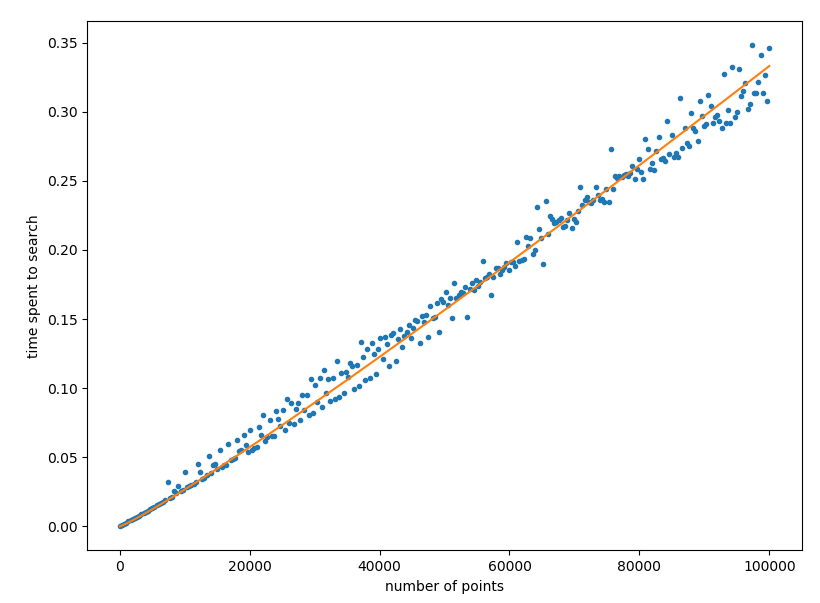
\includegraphics[width=\textwidth, height=8cm,keepaspectratio]{create_KDTree.png}
			\captionof{figure}{Create\_KDTree(\#pts vs time)\label{fig:img1}}
			
	  \par}
  		In the figure above, the blue dots represent the size of the vectors (the number of points they contain) (x-axis) and how much time it took to create their corresponding KDTrees (y-axis).
  		
  		As we can see from the plot, we were able to fit an nlog(n) curve to the points (where n is the number of points in the KDTrees) 
  		
  	\subsection{Find Nearest Neighbors}
  	
  		In this step, we tried to prove that it takes in average O(log n) in time to find the nearest neighbor to a given point. Therefore, we created 200 KDTrees following the same process described in the previous step. After that, we generated a random point for each KDTree (These points are not necessarily part of the KDTrees) and then we ran queries on the KDTrees to find the nearest neighbor to those random points. We recorded the processing time each time in order to plot the results and we obtained the following graph:
  		
  		{\centering
  			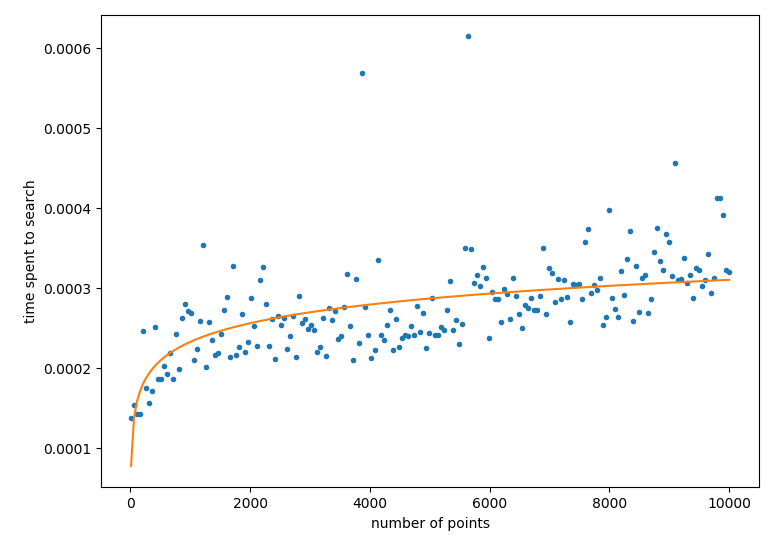
\includegraphics[width=\textwidth, height=8cm,keepaspectratio]{nearest_n.png}
  			\captionof{figure}{Find Nearest Neighbor(\#pts vs time)\label{fig:img1}}
  			
  			\par}
  		
  		As we can see from figure 2, we were able to fit a log(n) curve to the blue dots, which means that it takes in average log(n) (where n is the number of points in the KDTree)in time to find the nearest neighbor to a given point using the KDTree approach.
  		
  	\subsection{Find K Nearest Neighbors}
  		
  		This step is similar to the previous one, at the only difference that instead of trying to prove the time complexity of the algorithm to find only the nearest neighbor, we tried to prove it when looking for the 4 nearest neighbors. After generating the points and created the KDTrees as described in the previous step, we ran queries on KDTrees to find the 4 nearest neighbors to the randomly generated points. We recorded the processing times, plotted the results and obtained the following graph
  		
  		{\centering
  			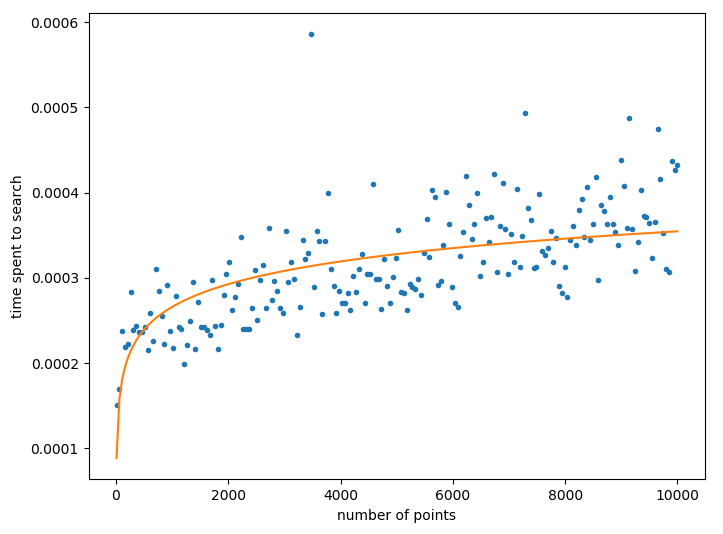
\includegraphics[width=\textwidth, height=8cm,keepaspectratio]{k_nearest_n.png}
  			\captionof{figure}{Find k Nearest Neighbors(\#pts vs time)\label{fig:img1}}
  			
  			\par}
  		
  		As we can see from figure 3, we were able to fit a log(n) curve to the blue dots, which means that it takes in average log(n) (where n is the number of points in the KDTree)in time to find the k nearest neighbors to a given point using the KDTree approach.
 \section{Visual Representation}
 		The graph below is just a visual representation of 10 randomly generated points (red dots) linked to their 3 nearest neighbors in a set containing 100 points (blue dots)
 		
 		{\centering
 			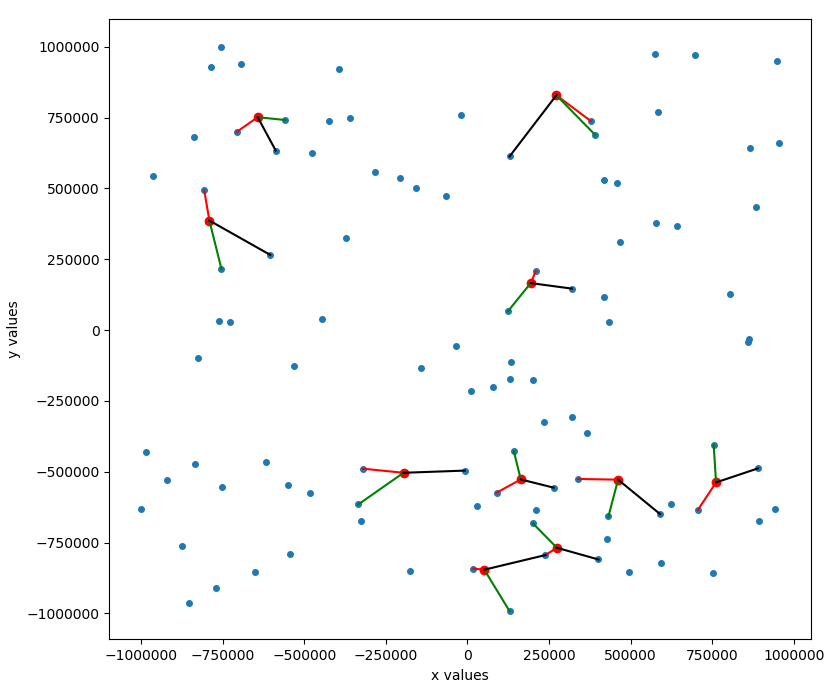
\includegraphics[width=\textwidth, height=8cm,keepaspectratio]{n_visual.png}
 			\captionof{figure}{k Nearest Neighbors Representation (x vs y)\label{fig:img1}}
 			
 			\par}
 		
 		In the figure above,
 		\begin{itemize}
 			\item The blue dots represent the points in the set
 			\item The Red dots are randomly generated points (we try to find their 3 nearest neighbors)
 			\item The red lines link the random points to their nearest neighbors
 			\item The green lines link the random points to their 2nd nearest neighbors
 			\item The black lines link the random points to their 3rd nearest neighbors
 		\end{itemize}
 \section{Conclusion}
 	In this report we were able to prove the time complexities related to the KNN problem using KDTrees as described in class. We proved that finding the KNNs to a given point can be done in O(log n), while it takes O(nlog n) to preprocess the initial data (basically construct the KDTree given a set of points) where n is the number of points in the set.
\end{document}
